\subsection{GRC analysis}
\label{sec:agrc-analysis}

%In order to statically determine the worst case memory consumption of a
%program targeting TP-JOP, one needs to analyze codes generated from both
%CNs and JDNs. The compiler is able to trivially determine the maximum
%memory footprint required for executing CN codes from any given SystemJ
%programs [] since there is no dynamic memory allocation required for
%executing this code. On the other hand, the data-flow analysis for JDNs
%is more intricate since it needs to analyze the original GRC in order
%to retrieve the dependency edges, which are lost after splitting CNs and
%JDNs from the GRC. We devote this section to illustrate this analysis
%technique.

GRC is a \textit{directed graph} $G =(V,E)$, where $V$ is the set of
vertices (nodes of GRC) and $E$ is the set of ordered pairs of
vertices. Each edge
$e = (v_i,v_j), \forall e \in E, v_i \in V, v_j \in V$ is a tuple
denoting that the edge is directed from $v_i$ to $v_j$.  Then a lambda
function $\lambda:v \rightarrow E_i$, $E_i \subseteq E$, maps
\textit{each} vertex to a set of edge(s) where $\forall (v_i,v) \in E_i$
and $E_i$ may be $\emptyset$. When $|E_i| = 1$ we call $v_i$
\textit{must} happen before $v$ whereas when $|E_i| > 1$ we say any
$v_i \in E_i$ \textit{may} happen before $v$.

\begin{figure}[t!]
	\newsavebox{\codeone}
	\begin{lrbox}{\codeone}
		\begin{minipage}[b]{0.62\textwidth}
		\begin{lstlisting}[tabsize=1,basicstyle=\small\ttfamily,numbers=left]
(mList 
	(mNode JDN1 (Must Null) (May Null))
	(mNode JDN2 
		(Must (mNode JDN1 (Must Null) (May Null))) 
		(May Null))
	(mNode JDN3 
		(Must (mNode JDN1 (Must Null) (May Null))) 
		(May Null))
	(mNode JDN4 (Must Null)
		(May 
			(mNode JDN2 
				(Must (mNode JDN1 (Must Null) (May Null))) 
				(May Null))
			(mNode JDN3 
				(Must (mNode JDN1 (Must Null) (May Null))) 
				(May Null))))
		\end{lstlisting}
	\end{minipage}
	\end{lrbox}

	\centering
	\subfloat[An abstracted GRC graph]{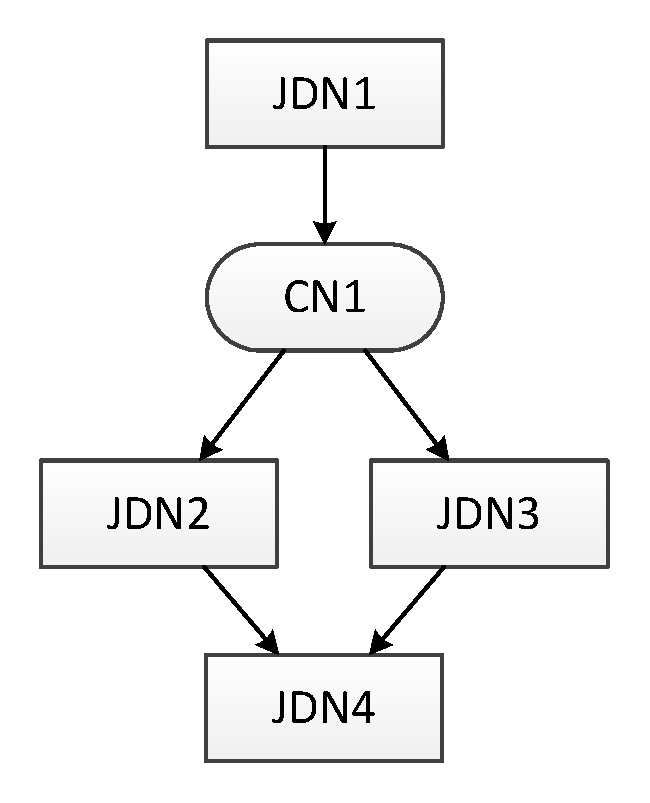
\includegraphics[scale=0.3]{may}
	\label{fig:aagrc}}
	\hspace{1.0cm}
	\subfloat[An output of the GRC
	analysis]{\scalebox{0.8}{\usebox{\codeone}}\label{fig:tttt}}
	\caption{An example of GRC analysis}
	\label{fig:maymust}
\end{figure}

In this section, we illustrate how the data-structure, which contains
information on the \textit{may} and \textit{must} relationships between
the nodes, is obtained from the GRC. Consider a snippet of GRC graph
shown in Figure~\ref{fig:aagrc}. Here, the root node, \texttt{JDN1}, has
no parent whereas it has an immediate child \texttt{CN1}. \texttt{CN1}
has two children, \texttt{JDN2} and \texttt{JDN3}, and both of these
JDNs have the same child \texttt{JDN4}. This graph when given as an
input to our GRC analysis tool, returns the result as a S-expression as
shown in Figure~\ref{fig:tttt}. The resultant recursive data-structure
consists of a set of nodes called \texttt{mNode}, which has three
fields: (1) the node name of type string, (2) \texttt{Must} field of
type \texttt{mNode} and (3) \texttt{May} field, which is a set of type
\texttt{mNode}. This data-structure can be used to identify potential
callers of each \texttt{JDN} in the GRC graph. For example, since
\texttt{JDN1} has no parents, its \texttt{Must} and \texttt{May} fields
are both \texttt{Null} (line 2).  On the other hand, \texttt{JDN1} must
be called before \texttt{JDN2} or \texttt{JDN3}, hence \texttt{Must} of
both \texttt{JDN2} and \texttt{JDN3} is \texttt{JDN1} (lines 4 and 7).
Lastly, \texttt{JDN4} has two parent nodes; \texttt{JDN2} and
\texttt{JDN3}. Therefore, its \texttt{May} field has both \texttt{JDN2}
and \texttt{JDN3} (lines 11-16). It should be noted that we are only
interested in callers of \texttt{JDNs}, hence \texttt{CNs} are not
included in the final result (Figure~\ref{fig:tttt}). % A complete
% algorithm of our GRC analysis is given in~\cite{supp_amal02916}.







%%% Local Variables:
%%% mode: latex
%%% TeX-master: "jgc_cc_pe"
%%% End:
